%%%%%%%%%%%%%%%%%%%%%%%%%%%%%%%%%%%%%%%%%
% Beamer Presentation
% LaTeX Template
% Version 1.0 (10/11/12)
%
% This template has been downloaded from:
% http://www.LaTeXTemplates.com
%
% License:
% CC BY-NC-SA 3.0 (http://creativecommons.org/licenses/by-nc-sa/3.0/)
%
%%%%%%%%%%%%%%%%%%%%%%%%%%%%%%%%%%%%%%%%%

%----------------------------------------------------------------------------------------
%	PACKAGES AND THEMES
%----------------------------------------------------------------------------------------

\documentclass{beamer}

\mode<presentation> {
	\usetheme{CambridgeUS}
	\setbeamertemplate{footline}[page number]
	\setbeamertemplate{navigation symbols}{}
}

\usepackage[utf8]{inputenc}
\usepackage[english,spanish]{babel}
\usepackage{graphicx} % Allows including images
\usepackage{booktabs} % Allows the use of \toprule, \midrule and \bottomrule in tables

%----------------------------------------------------------------------------------------
%	TITLE PAGE
%----------------------------------------------------------------------------------------

\title[Intelligence after CMI]{La noción de inteligencia después de\\ \textit{Computing Machinery and Intelligence}} % The short title appears at the bottom of every slide, the full title is only on the title page

\author{Pedro Montoto García\\Enrique Alonso González} % Your name
\institute[USC]{Universidade de Santiago de Compostela}
\date{}

\begin{document}

\begin{frame}
\titlepage % Print the title page as the first slide
\end{frame}

\begin{frame}
	\frametitle{El Juego de la Imitación: Alan Turing}
\begin{center}
    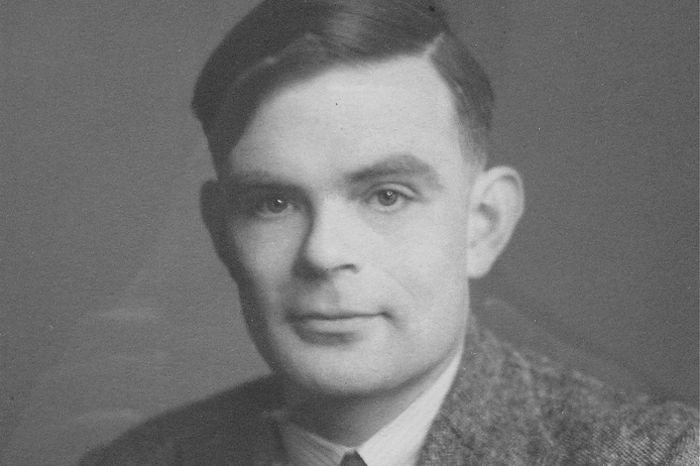
\includegraphics[width=0.7\textwidth]{turing}
    
    Alan M. Turing (1912-1954)
   
    \textit{¿Puede pensar una máquina?}: \textit{Computing Machinery and Intelligence}(1950)	
    
    
\end{center}
\end{frame}

\begin{frame}
	\frametitle{El Juego de la Imitación}
\begin{center}
    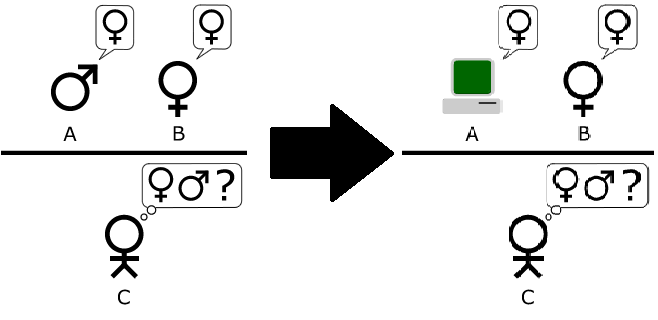
\includegraphics[width=0.7\textwidth]{imitation_game}
\end{center}
\end{frame}

%------------------------------------------------

\begin{frame}
\frametitle{Argumento por analogía}

Implícitamente:

\begin{center}
\textit{Si} una \textbf{máquina} \textit{puede hacerse pasar} por una \textbf{persona}, \\ una máquina puede \textbf{pensar} como una persona

\hfill
\hfill
\hfill
\hfill

\scalebox{3}{$\Uparrow$}

\hfill
\hfill
\hfill
\hfill

\textit{Si} un \textbf{hombre} \textit{puede hacerse pasar} por una \textbf{mujer}, \\ un hombre puede \textbf{pensar} como una mujer
\end{center}

\end{frame}

%------------------------------------------------

\begin{frame}
\frametitle{Premisas implícitas}
\begin{block}{Test Indirecto}
``Entre lenguaje y pensamiento existe una relación directa''
\end{block}

\begin{block}{Imitación}
``Ser capaz de imitar una característica es evidencia de poseer dicha característica'' 
\end{block}

\begin{block}{Subjetivismo}
``La identificación subjetiva de una característica es evidencia de poseer dicha característica''
\end{block}
\end{frame}

%------------------------------------------------

\begin{frame}
\frametitle{Resultados}
Aceptando las condiciones anteriores, el argumento de Turing resulta en:
\begin{center}
\textit{Si} una \textbf{máquina pasa el TT} dicha máquina es \textbf{capaz de pensar}
\end{center}

\end{frame}

%------------------------------------------------

\begin{frame}
\frametitle{Jerarquía de Tests de Turing (Harnad, 2000)}

\begin{footnotesize}
\begin{center}
\begin{tabular}{l | c | c}
    Objeción & & Nombre \\
    \hline
    & {\usebeamercolor[fg]{structure} t1} & Modelos de Juguete (Subconjuntos) \\
    & {\usebeamercolor[fg]{structure} T2} & Test de Turing tradicional y variantes \\
    Habitación China & {\usebeamercolor[fg]{structure} (ST)} & Variante Searleana del TT  tradicional \\
    Sensorimotor $\not =$ simbólico & {\usebeamercolor[fg]{structure} T3} & Total/Robot Turing Test \\
    + Equivalencia Microfuncional & {\usebeamercolor[fg]{structure} T4} & Human Robot Turing Test \\
    + Auto-preservación & {\usebeamercolor[fg]{structure} (T4+)} & Truly Total Turing Test\footnote{No recogido en el artículo} \\
    Teoría Total & {\usebeamercolor[fg]{structure} T5} & Imitación perfecta \\
\end{tabular}
\end{center}
\end{footnotesize}

\end{frame}


\begin{frame}
\frametitle{Otras objecciones: el método no es adecuado
}
\begin{itemize}
    \item Problema: Falsos positivos y negativos
    \begin{itemize}
        \item Ej: La máquina de pisar pies
        \item Ej: Inteligencias no humanas (test de gaviotas)
        \item Ej: Falibilidad humana (en imitación y detección)
        \item Causa: Un único test no es fiable
        \begin{itemize}
            \item Solución A: Múltiples jueces
            \item Solucion B: Test continuado/repetición en el tiempo
        \end{itemize}
    \end{itemize}
    \item Problema: Arbitrariedad
    \begin{itemize}
        \item Solución: Test estandardizado repetible
    \end{itemize}
\end{itemize}

\end{frame}

\begin{frame}
\frametitle{Conclusiones}

\begin{itemize}
    \item Limitaciones en forma y asunciones
    \begin{itemize}
        \item Siendo conscientes de ellas, pueden preverse errores
        \item La evaluación de cada caso de test permite mejorarlo (meta-evaluación)
    \end{itemize}
    \item Inteligencia como algo arbitrario
    \begin{itemize}
        \item Se hace necesaria una descripción fenomenológica
        \item El test debe incorporarla
    \end{itemize}
    \item Sin embargo, es una definición operativa
\end{itemize}

\end{frame}

%------------------------------------------------

\begin{frame}
\frametitle{Cierre y preguntas}
\Huge{\centerline{Gracias por su atención!}}
\end{frame}

%----------------------------------------------------------------------------------------

\end{document} 